\documentclass{beamer}

\usetheme{Frankfurt} 
\usecolortheme{seahorse}

\usepackage{graphicx}
\usepackage{hyperref}
\usepackage{xcolor}
\usepackage{listings}
\usepackage{multicol}
\usepackage{tikz}
\usepackage{animate}
\usepackage{fancyvrb}
\usepackage{tcolorbox}
\usepackage{caption}
\usepackage{booktabs}
\usepackage{lipsum} 
\definecolor{awsorange}{RGB}{255,153,0}
\definecolor{awsblue}{RGB}{24,104,183}
\definecolor{awsgreen}{RGB}{88,161,44}
\definecolor{lightgray}{gray}{0.9}


\setbeamercolor{itemize item}{fg=awsorange}
\setbeamertemplate{itemize item}[triangle]


\title{Amazon AWS: Cloud Computing Basics}
\subtitle{Understanding AWS Fundamentals}
\author{DK}
\institute{Ramakrishna Mission Vivekananda Centenary College}
\date{\today}


\setbeamersize{text margin left=1em, text margin right=1em}
\setlength{\leftmargini}{1.5em} % Adjust list indentation
\setlength{\rightskip}{0pt plus 1em} % Allow for flexible right margin
\setlength{\parindent}{0pt} 

\newtcolorbox[auto counter, number within=section]{mybox}[2][]{colback=lightgray, colframe=awsblue, 
fonttitle=\bfseries, title=#2 #1}

\begin{document}


\begin{frame}
    \titlepage
\end{frame}

% Slide: What is AWS?
\begin{frame}{What is AWS?}
    \begin{itemize}
        \item Amazon Web Services (AWS) is a comprehensive cloud computing platform provided by Amazon.
        \item It offers a wide range of services including computing power, storage, and databases.
        \item AWS is used by businesses of all sizes to deploy applications and services.
    \end{itemize}
\end{frame}

% Slide: How AWS Works
\begin{frame}{How AWS Works}
    \begin{itemize}
        \item AWS provides on-demand computing resources through a pay-as-you-go model.
        \item Users can access these resources via the internet, using a web interface or API.
        \item AWS data centers are located globally, ensuring high availability and low latency.
    \end{itemize}
    \pause
    \begin{tcolorbox}[colback=white, colframe=awsblue, sharp corners=south, boxrule=0.8mm]
    \textbf{Note:} AWS's global infrastructure includes multiple regions and availability zones to ensure reliability.
    \end{tcolorbox}
\end{frame}

% Slide: Why Use AWS?
\begin{frame}{Why Use AWS?}
    \begin{multicols}{2}
        \begin{itemize}
            \item \textbf{Scalability:} Easily scale resources up or down based on demand.
            \item \textbf{Cost-Effective:} Pay only for the resources you use, avoiding upfront costs.
        \end{itemize}
        \columnbreak
        \begin{itemize}
            \item \textbf{Reliability:} Benefit from AWS’s global infrastructure for high availability.
            \item \textbf{Security:} Utilize robust security features to protect your data and applications.
        \end{itemize}
    \end{multicols}
\end{frame}

% Slide: AWS Security Features
\begin{frame}{AWS Security Features}
    \begin{itemize}
        \item \textbf{Identity and Access Management (IAM):} Control access to AWS resources securely.
        \item \textbf{Encryption:} Encrypt data at rest and in transit to protect sensitive information.
        \item \textbf{Compliance:} AWS adheres to various compliance standards including GDPR, HIPAA, and more.
        \item \textbf{Security Groups:} Configure firewall rules to control traffic to your resources.
    \end{itemize}
    \pause
    \begin{mybox}[toprule=1mm, bottomrule=1mm, toptitle=1mm, bottomtitle=1mm]{Tip}
    Regularly review and update your security policies and access controls to stay ahead of potential threats.
    \end{mybox}
\end{frame}

% Slide: AWS Core Services (with table)
\begin{frame}{AWS Core Services}
    \begin{table}[]
    \centering
    \begin{tabular}{ll}
        \toprule
        \textbf{Category} & \textbf{Services} \\
        \midrule
        Compute & EC2, Lambda, Elastic Beanstalk \\
        Storage & S3, Glacier, EBS, EFS \\
        Database & RDS, DynamoDB, Aurora, Redshift \\
        Networking & VPC, Route 53, CloudFront \\
        \bottomrule
    \end{tabular}
    \caption{Key AWS Core Services}
    \end{table}
\end{frame}

% Slide: AWS Pricing Overview
\begin{frame}{AWS Pricing Overview}
    \begin{center}
        \animategraphics[autoplay,loop,width=0.7\textwidth]{5}{aws-pricing-}{1}{10}
    \end{center}
    \vspace{-1ex}
    \note{The animation above highlights the key elements of AWS pricing.}
\end{frame}

% Slide: AWS Services Architecture
\begin{frame}{AWS Services Architecture}
    \begin{center}
    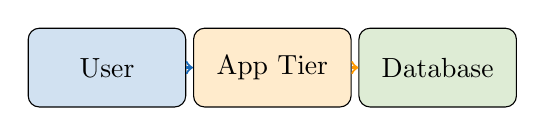
\begin{tikzpicture}[scale=0.7, every node/.style={text centered, minimum width=2cm, minimum height=1cm}]
        \node[draw, fill=awsblue!20, rounded corners] (user) at (0,0) {User};
        \node[draw, fill=awsorange!20, rounded corners] (app) at (3,0) {App Tier};
        \node[draw, fill=awsgreen!20, rounded corners] (db) at (6,0) {Database};
        
        \draw[->, thick, color=awsblue] (user) -- (app);
        \draw[->, thick, color=awsorange] (app) -- (db);
    \end{tikzpicture}
    \end{center}
\end{frame}

% Slide: Conclusion
\begin{frame}{Conclusion}
    \begin{itemize}
        \item AWS is a powerful cloud platform that provides a range of services to meet diverse business needs.
        \item Its scalable and cost-effective nature makes it a preferred choice for many organizations.
        \item AWS’s security features ensure that data and applications are protected.
    \end{itemize}
\end{frame}

% Slide: Thank You
\begin{frame}{Thank You}
    \begin{center}
        \Huge \textcolor{awsorange}{Thank You!}
    \end{center}
    \vspace{1cm}

\end{frame}

\end{document}